% --------------------------------------------------------------
% This is all preamble stuff that you don't have to worry about.
% Head down to where it says "Start here"
% --------------------------------------------------------------
 
\documentclass[11pt]{article}
 
\usepackage[margin=.65in]{geometry} 
\usepackage{amsmath,amsthm,amssymb,titlesec,changepage}
\usepackage{graphicx}
\usepackage{listings}
\usepackage{xcolor}
\usepackage{textcomp}
\usepackage{fixltx2e}
\lstset{ %
language=R,                % choose the language of the code
basicstyle=\footnotesize,       % the size of the fonts that are used for the code
numbers=left,                   % where to put the line-numbers
numberstyle=\footnotesize,      % the size of the fonts that are used for the line-numbers
stepnumber=1,                   % the step between two line-numbers. If it is 1 each line will be numbered
numbersep=5pt,                  % how far the line-numbers are from the code
backgroundcolor=\color{white},  % choose the background color. You must add \usepackage{color}
showspaces=false,               % show spaces adding particular underscores
showstringspaces=false,         % underline spaces within strings
showtabs=false,                 % show tabs within strings adding particular underscores
frame=single,           % adds a frame around the code
tabsize=2,          % sets default tabsize to 2 spaces
captionpos=b,           % sets the caption-position to bottom
breaklines=true,        % sets automatic line breaking
breakatwhitespace=false,    % sets if automatic breaks should only happen at whitespace
escapeinside={\%*}{*)}          % if you want to add a comment within your code
}

\newtheoremstyle{quest}{\topsep}{\topsep}{}{}{\bfseries}{}{ }{\thmname{#1}\thmnote{ #3}.}
\theoremstyle{quest}
\newtheorem*{definition}{Definition}
\newtheorem*{theorem}{Theorem}
\newtheorem*{question}{Question}
\newtheorem*{exercise}{Exercise}
\newtheorem*{challengeproblem}{Challenge Problem}

%% If you want to use a function like ''sin'' or ''cos'', you can do it like this
%% (we probably won't have much use for this)
% \DeclareMathOperator{\sin}{sin}   %% just an example (it's already defined)
%% If you want to define a new command, you can do it like this:
\newcommand{\problem}[1]{\section{#1}}        % Problem.
\newcommand{\subproblem}[1]{\subsection{#1}}      % Sub Problem
\newcommand{\subsubproblem}[1]{\subsubsection{#1}}      % Sub Problem
\newcommand{\N}{\mathbb{N}}
\newcommand{\Z}{\mathbb{Z}}
\newcommand{\Q}{\mathbb{Q}}
\newcommand{\R}{\mathbb{R}}
\newcommand{\C}{\mathbb{C}}
\newcommand{\Sup}{\textsuperscript}
\newcommand{\Sub}{\textsubscript}

% \setcounter{section}{-1}
\titleformat{\section}{\normalfont\Large\bfseries}{Problem \thesection}{1em}{}
\titleformat{\subsection}{\normalfont\it}{\hspace{1em}\bf\thesubsection}{1em}{}
\titleformat{\subsubsection}{\normalfont\it}{\hspace{1.5em}\bf\thesubsubsection}{1em}{}
\renewcommand{\thesubsubsection}{\thesubsection\alph{subsubsection}}
 
\begin{document}
 
% --------------------------------------------------------------
%                         Start here
% --------------------------------------------------------------
 
\title{Homework 3}
\author{\small{Jason Mann (jcm2207)}\\
\small{Statistical Machine Learning (STAT W4400)}}
\date{}
 
\maketitle


\problem{$l_q$ regression}

\subproblem{Does one/none/both of the cost functions encourage sparse estimates? If so, which one? Explain your answer.}
\begin{adjustwidth}{3.5em}{0em}
The cost function shown on the left will encourage sparse estimates due to the cost increasing slowly along the axes, which is shown by the extreme points of the cost function. i.e. points further from the origin can have a relatively low cost.
\end{adjustwidth}


\subproblem{Which of the points would achieve the smallest cost under the \textit{l\Sub{q}}-constrained least squares cost function? For each of the two cases, name the respective point and give a brief explanation for your answer.}
\begin{adjustwidth}{3.5em}{0em}
Left: \textit{x\Sub{3}} is the point with the least cost. \\
Right: \textit{x\Sub{4}} is the point with the least cost. \\
The figures drawn for the cost functions can be seen as contour lines for the cost function, and \textit{x\Sub{3}} on the left and \textit{x\Sub{4}} on the right both are on the closest contour to the origin.
\end{adjustwidth}




\problem{Combining Kernels}
\subproblem{Show that for any positive real number $a, k(x, x^{'}) := ak_1(x, x^{'})$ is a kernel}

\begin{adjustwidth}{3.5em}{0em}
If $a$ is positive, then $\sqrt{a}*\sqrt{a}=a$
\end{adjustwidth}
\begin{align*}
 \phi^{'}(x) &= \sqrt{a}\phi(x) \\
ak_1(x, x^{'}) &= a * <\phi(x), \phi(x^{'})> \\
&= a * \sum_i{\phi(x)_i\phi(x^{'})_i} = \sum_i{a\phi(x)_i\phi(x^{'})_i} \\
&= \sum_i{\sqrt{a}\phi(x)_i\sqrt{a}\phi(x^{'})_i} \\
&= \sum_i{ \phi^{'}(x)_i \phi^{'}(x^{'})_i} = <\phi^{'}(x), \phi^{'}(x^{'})> 
\end{align*}
\begin{adjustwidth}{3.5em}{0em}
Therefore because $ak_1(x, x^{'}) := <\phi^{'}(x), \phi^{'}(x^{'})>$ it follows that $k(x,x^{'})$ is a kernel
\end{adjustwidth}


\subproblem{Show that $k(x, x^{'}) := k_1(x, x^{'})k_2(x, x^{'})$ is a kernel}
\begin{align*}
k(x, x^{'}) &= k_1(x, x^{'})k_2(x, x^{'}) \\
 			&= <\phi_1(x), \phi_1(x^{'})><\phi_2(x), \phi_2(x^{'})> \\
 			&= \sum_i{\phi_1(x)_i\phi_1(x^{'})_i} * \sum_i{\phi_2(x)_i\phi_2(x^{'})_i} \\
 			&= \sum_i{\phi_1(x)_i\phi_2(x)_i\phi_1(x^{'})_i\phi_2(x^{'})_i} \\
\phi^{'}(x) &= \phi_1(x)\phi_2(x) \\
k(x, x^{'}) &= \sum_i{ \phi^{'}(x)_i \phi^{'}(x^{'})_i} = <\phi^{'}(x), \phi^{'}(x^{'})> 
\end{align*}


\subproblem{Show that for any positive integer $p, k(x, x^{'}) := k_1(x, x^{'})^p$ is a kernel}
\begin{adjustwidth}{3.5em}{0em}
Because we know that $k(x, x^{'}) := k_1(x, x^{'})k_2(x, x^{'})$ is a kernel from above, we can build kernels from successive multiplications of $k_1$, i.e. $k_2(x, x^{'}) = k_1(x, x^{'})k_1(x, x^{'}), ...\; k_p(x, x^{'}) = k_{p/2}(x, x^{'})k_{p/2}(x, x^{'})$. If p is even then $k(x, x^{'}) := k_{p/2}(x, x^{'})k_{p/2}(x, x^{'})$ and $k(x, x^{'}) := k_{p-1}(x, x^{'})k_{1}(x, x^{'})$ if p is odd. Therefore if $k_1$ is a kernel, then k is also a kernel.
\end{adjustwidth}





\vspace{1em}
\problem{Boosting}

\subproblem{Implement the AdaBoost algorithm in R.}
\begin{adjustwidth}{3.5em}{0em}  
\begin{lstlisting}

# Implementation of simple iterative adaboost algorithm
# train_data: training data (row is a data point combined with class label)
# test_data: test data same format as training data
# train: training method for weak learner
# classify: classification method for weak learner
# B: number of weak learners to train
adaboost <- function(train_data, train, classify, B, test_data=list()) {
    X <- train_data$X
    y <- train_data$y
    n <- nrow(X)
    # initialize weights to even distribution
    w <- rep(1/n,n)

    # initialize returns
    classifiers <- matrix(nrow=0,ncol=3)
    training_errors <- vector()
    alphas <- vector()
    test_errors <- vector()
    agg_training_errors <- vector()
    agg_test_errors <- vector()

    # progress bar
    pb <- create_progress_bar("text")
    pb$init(B)
    for(b in 1:B) {
        # train a weak learner on the weighted data
        classifier <- train(X, w, y)
        # classify data with weak learner
        y_prime <- classify(X, classifier)
        # compute the error of the weak learner
        error <- classifier_error(y, y_prime, w=w)

        # compute voting weights
        alpha <- log(1/error) - .1 * ifelse(b>1,alphas[b-1],1)

        # recompute weights
        for(i in 1:n) {
            if(y[i] != y_prime[i]) w[i] <- w[i] * exp(alpha)
        }

        # store data
        classifiers <- rbind(classifiers, classifier)
        training_errors <- c(training_errors,error)
        alphas <- c(alphas,alpha)

        if(length(test_data) > 0){
            # single classifier test error
            y_prime <- classify(test_data$X, classifier)
            test_errors <- c(test_errors,classifier_error(test_data$y, y_prime))
            
            # aggregated training and test error
            y_prime <- aggregate_weak_classifiers(X, alphas, classifiers, classify)
            agg_training_errors <- c(agg_training_errors, classifier_error(y, y_prime))
            y_prime <- aggregate_weak_classifiers(test_data$X, alphas, classifiers, classify)
            agg_test_errors <- c(agg_test_errors, classifier_error(test_data$y, y_prime))
        }
        pb$step()
    }
    cat('\n')

    # return weights and parameters of weak learners
    return(list(classifiers=classifiers,alphas=alphas,
            training_errors=training_errors,test_errors=test_errors,
            agg_training_errors=agg_training_errors,
            agg_test_errors=agg_test_errors))
}

\end{lstlisting}
\end{adjustwidth}



\subproblem{Implement the train and classify functions for decision stumps.}
\begin{adjustwidth}{3.5em}{0em}  
\begin{lstlisting}

# Weak Learner function (Decision Stump)
# 
# X: a dataframe containing training data points
# w: vector containing the weights for each training vector x
# y: vector containing class labels for each training vector x
# return: a list which contains the parameters specifying the resulting 
#   classifier, here a triplet (j, theta, m) specifying the decision stump
# 
train_decision_stump <- function(X, w, y) {
    # get dimensions
    d <- ncol(X)
    n <- nrow(X)
    
    best_score <- 0
    best_j <- 1
    best_theta <- 0

    for(j in 1:d) {
        # re-initialize score for each dimension
        score <- 0

        # sort indicies based on dimension so that we can find the
        # optimal split in linear time
        indicies <- order(X[,j])
        last_i <- indicies[1]
        # iterate over sorted indicies, and modify the score by the weighted
        # class values updating the model if the best score is surpassed
        # Achieves optimal split in O(nd)
        for(i in indicies[2:n]) {
            score <- score - 2*w[i]*y[i]
            if(X[i,j] != X[last_i,j] && abs(score) > abs(best_score)) {
                best_score <- score
                best_j <- j
                best_theta <- (X[i,j] + X[last_i,j]) / 2
            }
            last_i <- i
        }
    }

    return (c(best_j, best_theta, sign(best_score)))
}


# Applies a Weak learner to the data and gives class labels
# 
# X: the training data (rows are vectors of the data)
# pars: the result of a training function, here a triplet specifying decision
#   stumps (j, theta, m)
classify_decision_stump <- function(X, pars) {
    n <- nrow(X)
    j <- pars[1]
    theta <- pars[2]
    m <- pars[3]
    # initialize class labels
    y_prime <- vector(mode='numeric',length=n)

    for(i in 1:n) {
        y_prime[i] <- ifelse(X[i,j] > theta, m, -m)
    }
    return(y_prime)
}



# X: training data (rows are vectors of points)
# alphas: denotes the vector of voting weights
# classifiers: contains the parameters of all the weak learners
# return: classification labels for data
aggregate_weak_classifiers <- function(X, alphas, classifiers, classify) {
    classifiers <- as.matrix(classifiers)
    n <- nrow(X)
    B <- nrow(classifiers)
    y_prime <- vector(mode='numeric', length=n)
    y_votes <- matrix(nrow=B, ncol=n)

    for(b in 1:B) {
        y_votes[b,] <- classify(X,classifiers[b,])
    }
    for(i in 1:n) {
        weighted_class <- 0
        for(b in 1:B) {
            weighted_class <- weighted_class + alphas[b] * y_votes[b,i]
        }
        y_prime[i] <- sign(weighted_class)
    }
    return(y_prime)
}
\end{lstlisting}
\end{adjustwidth}


\subproblem{Run your algorithm on USPS data with cross validation.}
\begin{adjustwidth}{3.5em}{0em}  
\begin{lstlisting}
run_kfold_adaboost <- function(X, y, B, K) {
    # data <- cbind(data.frame(y),data.frame(X))
    idxs <- sample(1:nrow(X), nrow(X) * 0.8, replace=FALSE)
    test_data <- list(X=X[-idxs,], y=y[-idxs])
    train_data <- list(X=X[idxs,], y=y[idxs])
    tr_folds <- split_k_fold(train_data$X, train_data$y, K)

    errors <- list(test=matrix(nrow=0,ncol=B),train=matrix(nrow=0,ncol=B))

    classifiers <- list()
    best_class <- NA
    best_error <- 1

    pb <- create_progress_bar("text")
    pb$init(K)
    for(k in 1:K) {
        tr_fold <- list(X=subset(tr_folds$X, (tr_folds$folds != k)),
                        y=subset(tr_folds$y, (tr_folds$folds != k)))
        test_fold <- list(X=subset(tr_folds$X, (tr_folds$folds == k)),
                        y=subset(tr_folds$y, (tr_folds$folds == k)))

        result <- adaboost(tr_fold, train_decision_stump,
            classify_decision_stump, B, test_fold)

        classifiers <- c(classifiers,list(as.matrix(cbind(result$classifiers,result$alphas))))
        # max_idx <- order(result$agg_test_errors)[1]
        if(result$agg_test_errors[length(result$agg_test_errors)] < best_error) {
            best_class <- list(classifiers=result$classifiers,
                                alphas=result$alphas)
            best_error <- result$agg_test_errors
        }

        length(result$agg_test_errors) <- B
        length(result$agg_training_errors) <- B
        errors$test <- rbind(errors$test,result$agg_test_errors)
        errors$train <- rbind(errors$train,result$agg_training_errors)

        pb$step()
    }

    test_data$y_prime <- aggregate_weak_classifiers(test_data$X, best_class$alphas, 
                        best_class$classifiers, classify_decision_stump)
    test_data$error <- classifier_error(test_data$y, test_data$y_prime)
    return(list(errors=errors, classifiers=classifiers,
                best_class=best_class, final_error=test_data$error))
}
\end{lstlisting}
\end{adjustwidth}


\vspace{4em}

\subproblem{Plot the training error and the test error as a function of b}
\begin{center}
Basic Adabost, final test error on 20\% test set with 100 iterations: 0.05
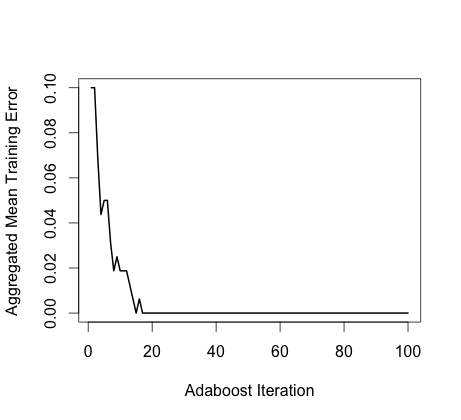
\includegraphics[width=.49\textwidth]{agg_basic_test}
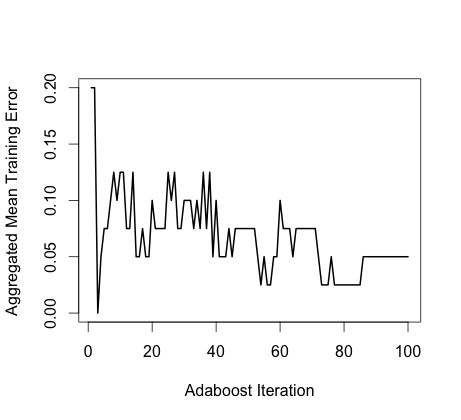
\includegraphics[width=.49\textwidth]{agg_basic_train}\\
AdaBoost with 5-Fold cross validation, final error on 20\% test set with 100 iterations: 0.025
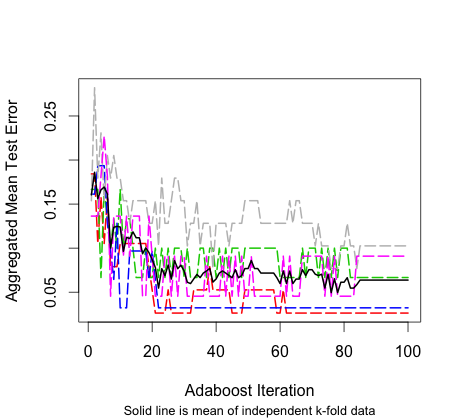
\includegraphics[width=.49\textwidth]{agg_kfold_test}
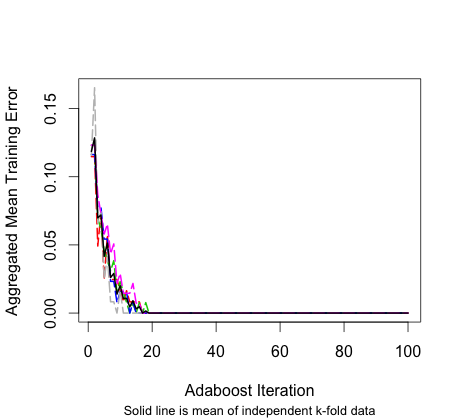
\includegraphics[width=.49\textwidth]{agg_kfold_train}\\
\end{center}
\begin{lstlisting}
run_adaboost <-function() {
    source('utils.r')
    X <- data.frame(read.table('uspsdata.txt'))
    y <- scan('uspscl.txt')

    results <- run_basic_adaboost(X,y,10)
    kfold_results <- run_kfold_adaboost(X,y,100,5)


    plot(lowess(results$errors$agg_train), type='l')
    plot(lowess(results$errors$agg_test), type='l')
    matplot(t(kfold_results$errors$train), type='l', xlab='Adaboost Iteration',ylab='Aggregated Mean Training Error', lty=5,lwd=2, col=c(2,3,4,8,6))
    lines(colMeans(kfold_results$errors$train),lwd=2)
    title(sub='Solid line is mean of independent k-fold data', cex.sub=.8)
    matplot(t(kfold_results$errors$test), type='l', xlab='Adaboost Iteration',ylab='Aggregated Mean Test Error', lty=5,lwd=2, col=c(2,3,4,8,6))
    lines(colMeans(kfold_results$errors$test),lwd=2)
    title(sub='Solid line is mean of independent k-fold data', cex.sub=.8)
}
\end{lstlisting}

%%%% don't delete the last line!
\end{document}